% You should title the file with a .tex extension (hw1.tex, for example)
\documentclass[a4paper, 11pt]{article}

\usepackage{amsmath}
\usepackage{amssymb}
\usepackage{fancyhdr}
\usepackage{graphicx}

\usepackage[margin=1in]{geometry}

\newcommand{\question}[2] {\vspace{.25in} \hrule\vspace{0.5em}
\noindent{\bf #1: #2} \vspace{0.5em}
\hrule \vspace{.10in}}
\renewcommand{\part}[1] {\vspace{.10in} {\bf (#1)}}

\newcommand{\myname}{Natthakan Euaumpon}
\newcommand{\myemail}{natthakaneuaumpon@gmail.com}
\newcommand{\myhwnum}{3}

\setlength{\parindent}{0pt}
\setlength{\parskip}{5pt plus 1pt}
 
\pagestyle{fancyplain}
\lhead{\fancyplain{}{\textbf{HW\myhwnum}}}      % Note the different brackets!
\rhead{\fancyplain{}{\myname\\ \myemail}}
\chead{\fancyplain{}{ICCS313 }}

\begin{document}

\medskip                        % Skip a "medium" amount of space
                                % (latex determines what medium is)
                                % Also try: \bigskip, \littleskip

\thispagestyle{plain}
\begin{center}                  % Center the following lines
{\Large ICCS313: Assignment \myhwnum} \\
\myname \\
\myemail \\
October 2019\\
\end{center}

\question{1}{Problem1}
There are 2 things we need to check. According to the theorem in lecture 4, if an undirected graph G is a tree it need to be:\\
1.The graph need to be connected\\
2.It must not contain a cycle\\
3.It has $n-1$ edges\\
If 2 of the three condition are true, then an undirected graph G is a tree. For this algorithm we will prove by using the first and the second condition which will then implies that the third condition is correct.\\
Assume $G$ is connected and doesn't contain a cycle. We are going to show this by induction.
Assume (3) is true for any graph < $n$ nodes. Consider $G$ with $n$ nodes. Pick any edge $e$ in $G$. Removing $e$ breaks $G$ into two components: $G_{1}$ and $G_{2}$. with $n_{1}$ and $n_{2}$ nodes respectively. Note that $n_{1} + n_{2} = n$. We know that $G_{1}$ and $G_{2}$ are connected and don’t contain any cycle. By IH, we know that $G_{1}$ has $n_{1} - 1$ edges and $G_{2}$ has $n_{2} - 1$ edges. So, $G$ has $(n_{1} - 1) + (n_{2} - 1) + 1 = n - 1$ edges.
The code is:\\
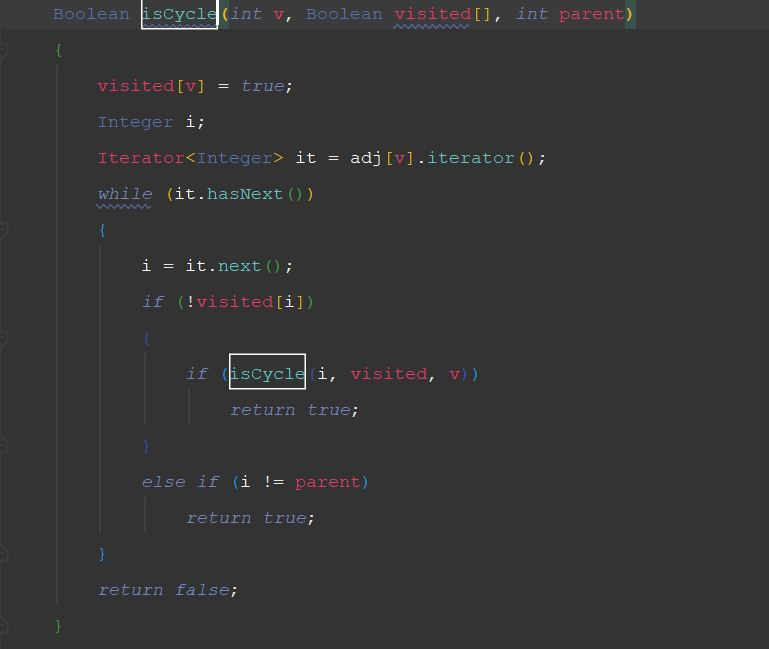
\includegraphics[width=\textwidth]{isCycle.jpg}\\
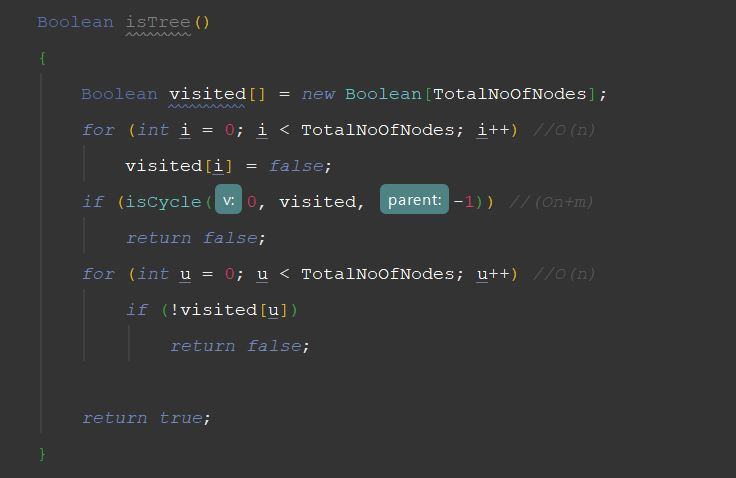
\includegraphics[width=\textwidth]{isTree.jpg}\\
To proof the code:\\
The isCycle will check whether the sub-graph is reachable for vertex v. It is recursively called function that will detect for any cycle. Firstly it will mark current node as visited. Then it will loop for any vertex that is connected to node v. If it is not visited it will recursively check for that vertex as well. The else if statement make sure that if the adjacent vertex is visited but is not the parent nodes its contain a cycle and return true immediately. Else if ir exit the while loop it will return false. This function will make sure that the second condition is True.\\
The isTree function will return true if the graph is connected and if isCycle is false. This algorithm check for cycle by calling the isCycle function and it check for connectivity as it return false immediately if it is not reachable which means it is not connected.This means that the algorithm is true as if fits the theorem and prove above.\\
Time Complexity:\\
Let n be the total number of vertices and , be the total number of edges. The first for loop in isTree function take $O(n)$ time. The if statement call the isCycle function. This takes $O(n+m)$ time. The last for loop take $O(n)$ time as we can check the if statement in $O(1)$ time complexity. So the total time complexity for this algorithm is $O(n) + O(n+m) + O(n) = O(n+m)$.\\
\question{2}{Problem2}
Proof by contradiction. Assume for the sake of contradiction that G is a DAG and every node has at least one entering edge and at least one outgoing edge. Pick a node v and follow edges backwards from v. We can do this since v has at least one entering edge (u, v). So we can walk backward to u. Again, we can repeat the
same argument about u and follow the edge (x, u) back to x. We keep doing this until we visit the same node twice, say w. We know that this will happen because we only have n nodes in total.\\
On the other hand every node have at least one outgoing edge. Pick a node n and follow edges forward from n. We can do this since n has at least one outgoing edge (n,m). So, we can walk forward to m. Again we can repeat the same argument about m and follow the edge (m,o) to m. We keep doing this we visit the same node twice, say z. We know that this will happen because we only have k nodes in total.\\
Let C be the sequence of nodes from w $->$ w. We have that C is a cycle. Thus, G is not a DAG. Hence, a contradiction.
\question{3}{Problem3}
Assume G is not connected, this means that there are 2 connecting component $G_{1}$ and $G_{2}$. Let u be the vertices for $G_{1}$ and v be vertices for $G_{2}$. Then the number of edges for $G_{1}$ and $G_{2}$ can be at most $\frac{(u-1)\cdot (u-2)}{2} + \frac{(v-1) \cdot (v-2)}{2}$. As $u + v = n$, so we can have at most $\frac{n^{2} - 2u \cdot (n-u) - (3n-4)}{2}$ edges. Since $1 < u < n$ which is less than $\frac{n^{2}}{2}$ this mean the total number of edges must be $\frac{n^{2}}{2}$ to have a degree of $\frac{n}{2}$ so there must be a vertex of degree less than $\frac{n}{2}$. So this means G is connected. Hence the statement is True.
\question{4}{Problem4}
The objective function is to sort for the customer with the least service time first.\\
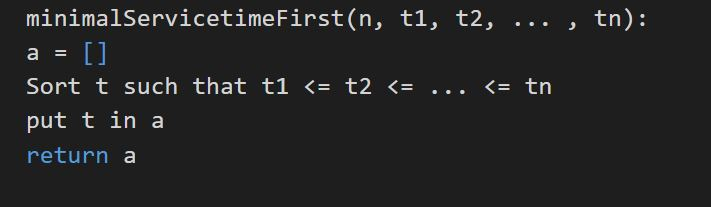
\includegraphics[width=\textwidth]{P4.jpg}\\
Observation: Customer with lesser service time will be serve first. Customer $t_{i}$ will be serve before customer $t_{j}$ where $i < j$.\\
Proof:\\
$$T = \sum_{i=1}^{n} \cdot  (\sum_{j=1}^{i} t_{j})$$\\
$T = t_{1} + (t_{1} + t_{2}) + ... + (t_{1} + t_{2} + ... + T_{n})$\\
$T = t_{1} \cdot n + t_{2} \cdot (n-1) + ... + t_{n}$\\
We can say that $t_{1} \leq t_{2} \leq ... \leq t_{n}$. As we sorted according to minimal service time.
\question{5}{Problem5}
\part{a}\\
Goal: Invite as many people as possible.\\
Constraint: Each people who has been invited must have at least 5 people whom they know.\\
As we can invite unlimited amount of people as long as they all fit in the constraint.\\
Objective: Remove people who should not be invited to the party (people that do not fit with the constraint).\\
Algorithm:\\
Construct a graph. Let a graph be G where n is vertices and m is edges. This algorithm will check every nodes. while walking down the graph G it will check whether a node has degrees of less than 5 or not. If it has a degree of less than 5 we append it into the created list L. Where it keep track of the nodes that do not qualify to attend the party. After eliminated a node there might be a new node with degree of less than 5. This is because the person who have a degree of 5 might a person that has been eliminated. This algorithm will run and check again to find unqualified nodes. The algorithm can keep track of this as it remove the edges connect with the node in L from its neighbour. After it checks all of the node it will return a list of qualified people who can be invite to the party.\\
Theorem: This algorithm is correct as it will gives the maximum number of people Alice can invite to her party.\\
Observation1: the algorithm will remove people who do not fit the above constraint.\\
Observation2: The list L will only contain unqualified people.\\
Proof:\\
The second observation make sure that no qualified people will we added to L. Since we have removed all unqualified people according to the first observation, we will have the maximum total number of qualified people with no unqualified people. Hence the Theorem holds.

\part{b}\\
Algorithm:\\
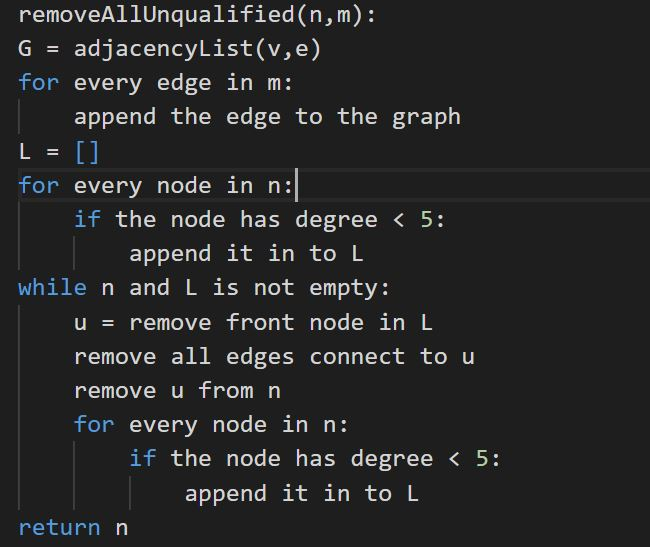
\includegraphics[width=\textwidth]{P5.jpg}\\
Where n is a list and L is queue of unqualified nodes.\\
Time complexity:\\
Construct a graph take O(m) time. The first for loop iteration take O(n) time as it take O(1) to enqueue the element, looking for element also take O(q) as we only look for the size. For the second iteration of for loop, we keep dequeue the first element out and removing the edges. This results in O(deg(u)) time complexity as we remove every edges that join with the disqualify node. Where u is a node in L and edges remove is its neighbour. As the size of n keep decreasing every time the iteration is finish it will take O(r(n+deg(u))) where r is the total number of removed nodes, u is node in L and n is the node we need to check. The return statement only take O(1) time complexity.\\
So the total run time is:\\
$O(m) + O(n) + O(r\cdot(n+deg(u)))$\\
$= O(m+n) + O(r\cdot(n+deg(u)))$
$O(r(n+deg(u)))$ is the most expensive when there is an unqualified nodes.\\
Best case:\\
$O(n+m)$ as there is no unqualified node so it does not need to go in to the while loop.\\
Worst case:\\
$O(n(n+deg(u)))$, which is equivalent to $O(n^{2} + n\cdot deg(u))$ as there are no one who fit with the constraint so we keep removing every node which is the biggest possible value of r.
\question{6}{Problem6}
My email is natthakan.eua@student.mahidol.edu\\
My username is Natthakan\\
Problem done: A, B, C and D
\end{document}

